\chapter{\library{dEchorate}: Datasets for Acoustic Echo Estimation}\label{ch:dechorate}

\openepigraph{Once you've been alone\\
And everybody knows\\
Work begins alone}{Strapping Young Lad, \textit{Monument}}


\vspace{-2.5em}
\newthought{Synopsis} \marginpar{%
\footnotesize
\textbf{Keywords:} Room impulse response, early reflection, acoustic echoes, audio database, microphone arrays.
\\\textbf{Resources:}
\begin{itemize}
    \item \href{https://github.com/Chutlhu/DechorateDB}{Code repository}
    \item \href{https://github.com/Chutlhu/DechorateDB}{Dataset data}
\end{itemize}
} \synopsisChDechorate


\mynewline
The material presented in the chapter is the result of a work done while visiting prof. Sharon Gannot and ing. Pinchas Tandeitnik at the Bar'Ilan University, Israel.
The work described here, together with its continuation described in~\cref{ch:dechorateapp} will be submitted as a journal article to the EURASIP special edition \textit{Data-driven Audio Signal Processing: Methods and Apps}.


\section{Introduction}\label{sec:dechorate:intro}
As discussed~\cref{sec:estimation:datasets}, many \acp{RIR} datasets are available online.
However, most of them are specifically designed for applications either to \acf{SE} or to \acf{RooGE}.
The main common drawback of these datasets in that they can not be easily used for other tasks than the one which they were designed for.
In particular, \SE/-oriented datasets lack of a proper annotation of echoes in the \acp{RIR} or the absolute position of objects inside the room.
Conversely, datasets for \RooGE/ typically features design choices which are not suitable for many \SE/ application, involving the positioning of microphone(s) and source(s).
\dEchorate{} was designed to fill this gap: a fully calibrated multichannel \ac{RIR} database with accurate annotation of the geometry and echoes in different configurations of a cuboid rooms with varying wall acoustic profiles.
The database currently features 1800 annotated \acp{RIR} obtained from 6 arrays of 5 microphones each, 6 sound sources in 10 different acoustic conditions.
All the measurements were realized in the acoustic lab at Bar-Ilan university following a consolidated protocol previously established for the realization of two other multichannel \acp{RIR} databases:
the \href{http://www.eng.biu.ac.il/~gannot/RIR_DATABASE/}{BIU's Impulse Response Database\ExternalLink} \citeonly{Hadad2014multichannel} gathering \acp{RIR} of different reverberation levels sensed by uniform linear arrays (ULAs);
and \href{https://asap.ite.tul.cz/downloads/MIRaGe/}{\library{MIRaGE}\ExternalLink}~\citeonly{cmejla2019mirage} providing a set of measurements of a source placed on a dense position grid.
\dEchorate{} is designed for \acf{AER} with linear arrays, and is more generally aimed at analyzing and benchmarking RooGE and echo-aware signal processing methods on real data.
In particular, it can be used to assess robustness against the number of reflectors, the reverberation time, additive spatially-diffuse noise and non-ideal frequency and directive characteristics of microphone-source pairs and surfaces in a controlled way.
Due to the amount of data and recording conditions, it could also be used to train machine learning models or as a reference to improve \ac{RIR} simulators.
The database is accompanied with a Python toolbox that can be used to process and visualize the data, to perform analysis or to annotate new datasets.

\begin{figure}[t]
    \begin{fullwidth}
        \centering
        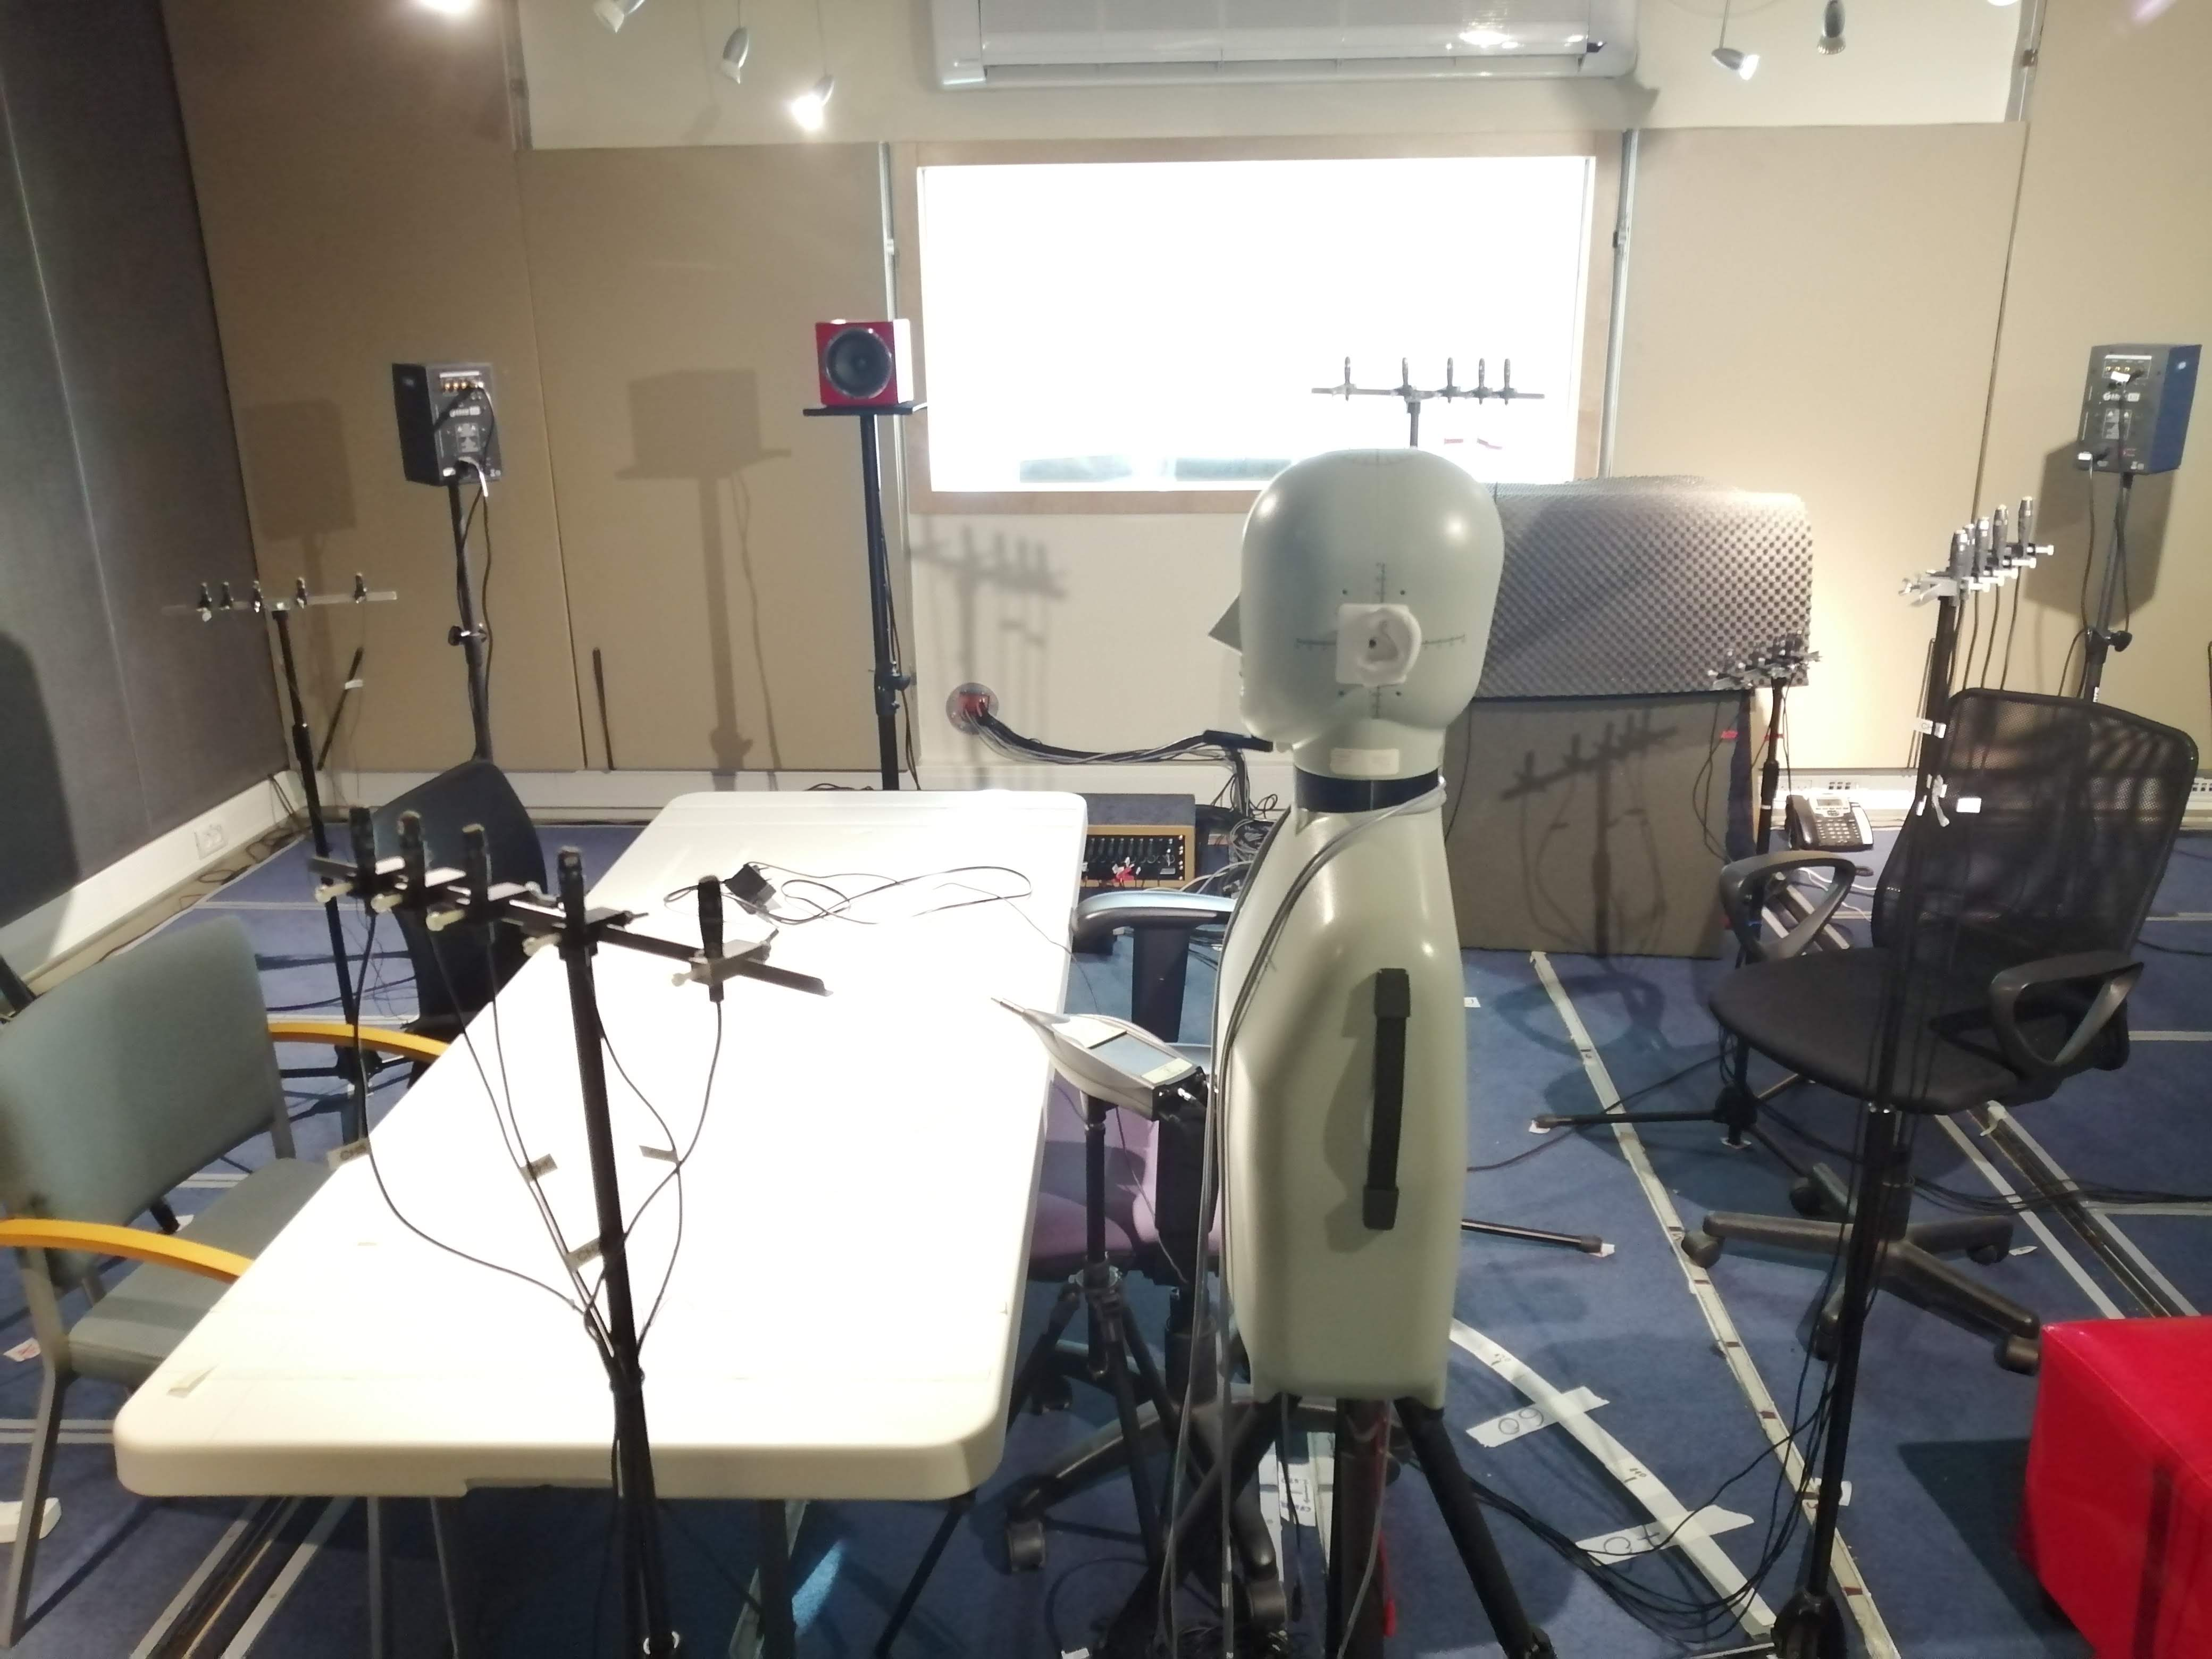
\includegraphics[trim={0 0 0 10em},clip,width=\linewidth]{dechorate/fornitures.jpg}
        \caption{Broad-view picture of the acoustic lab at Bar-Ilan university.}
        \label{fig:dechorate:room}
    \end{fullwidth}
\end{figure}


\section{Database realization}
\subsection{Recording setup}
The recording setup is situated in a cuboid room with dimension 6~m $\times$ 6~m $\times$ 2.4~m.
The 6 facets of the room (walls, ceiling, floor) are covered by acoustic panels allowing controllable reverberation time ($\RT$).
We placed $4$ directional loudspeakers (direct sources) facing the center of the room and $30$ microphones mounted on 6 non-uniform linear arrays (nULA) of 5 sensors each.
An additional channel is used for the loop-back signal, which serves to compute the time of emission and detect errors.
Each loudspeaker and each array was positioned close to one of the walls in such a way that the nature of the strongest echo can be easily identified.
Moreover, their positioning was chosen to cover a wide distribution of source-to-receiver distances, hence, a wide range of direct-to-reverberant ratios (\ac{DRR}).
Further, $2$ more loudspeakers were positioned pointing towards the walls (indirect sources).
This was done to study the case of early reflections being stronger than the direct-path.
Each linear microphone array consists of 5 microphones with non-uniform inter-microphone spacings of $[4, 5, 7.5, 10]$~cm\sidenote{
    \scriptsize\ie/
    $[-12.25, -8.25, $ $-3.25, 3.25, 13.25]$ cm w.r.t the barycenter}.
Each array is steered towards a different vertical edge of the room for calibration and reproducibility purposes.


\begin{table}[h]
    \begin{sidecaption}[]{
        Technical specification of the measurements equipment used in the recordings.
        }[tab:dechorate:room_equipment]
        \centering
        \small
        \begin{table}[]
    \centering
    \small
    \begin{tabular}{ll}
        \toprule
         Loudspeakers   & (directional, direct) $4 \times$ Avanton\\
                        & (directional, indirect) $2 \times$ Avanton\\
                        & (omnidirectional) $1 \times$ B\&G\\
                        & (babble noise) $4 \times$ 6301bx Fostex\\
         \hline
         Microphones    & $30 \times$ AKG CK32\\
         Array          & $6 \times$ nULA (5 mics each, handcrafted)\\
         \hline
         A/D Converter  & ANDIAMO.MC\\
         \hline
         Indoor Positioning & Marvelmind Starter Set HW v4.9\\
         \bottomrule
    \end{tabular}
    \caption{Measurements equipment.}
    \label{tab:room_equipment}
\end{table}
    \end{sidecaption}
\end{table}

\begin{figure}[b]
    \begin{sidecaption}[]{
        Illustration of the recording setup - top view.
        }[fig:dechorate:2D]
        \centering
        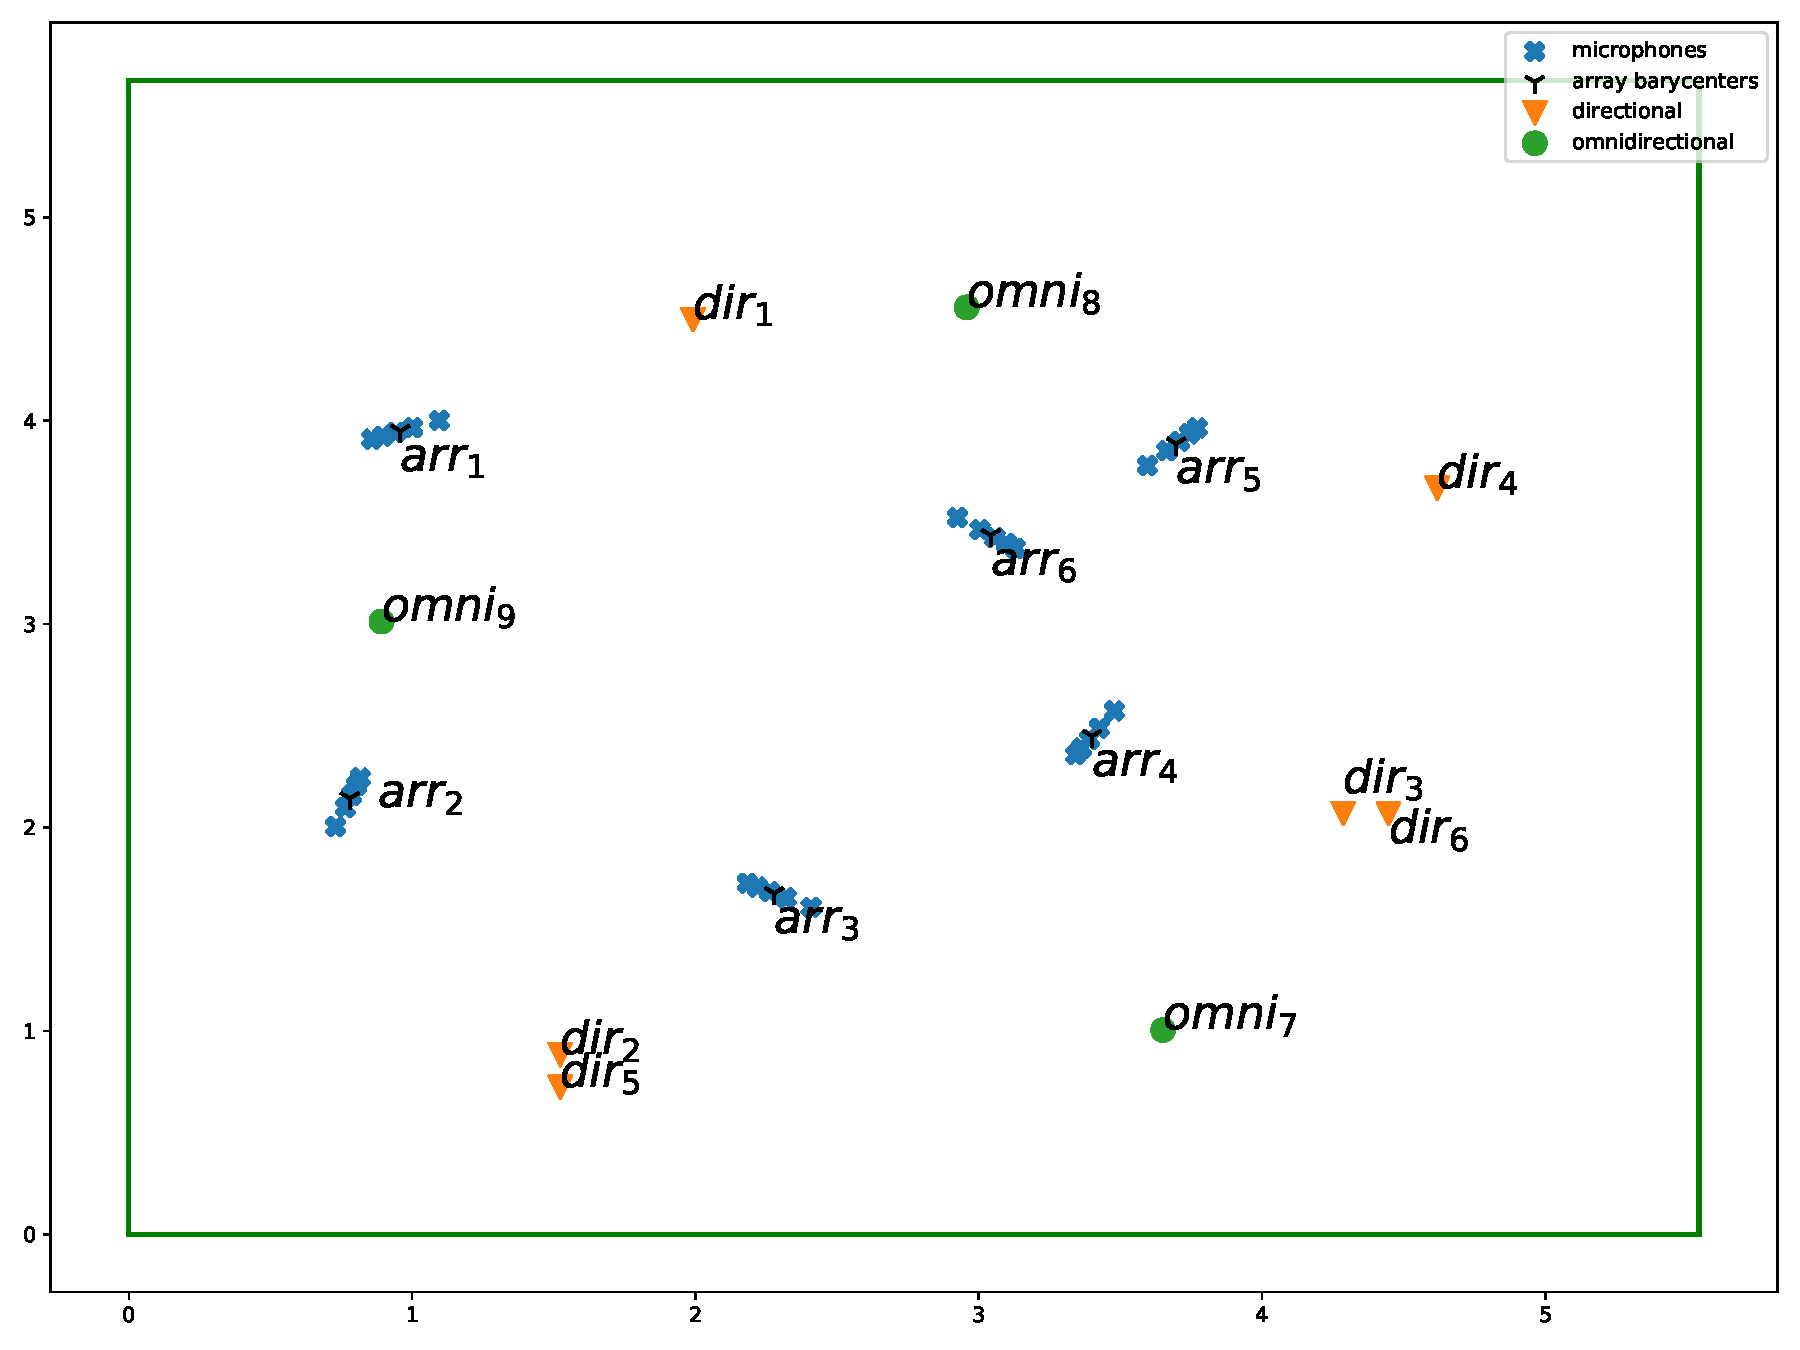
\includegraphics[width=0.8\linewidth]{figures/dechorate/positioning2D_xy.pdf}
    \end{sidecaption}
\end{figure}

\begin{figure}[t]
    \begin{fullwidth}
    \centering
    \subfloat[mu_spkr][Overall setup]{
        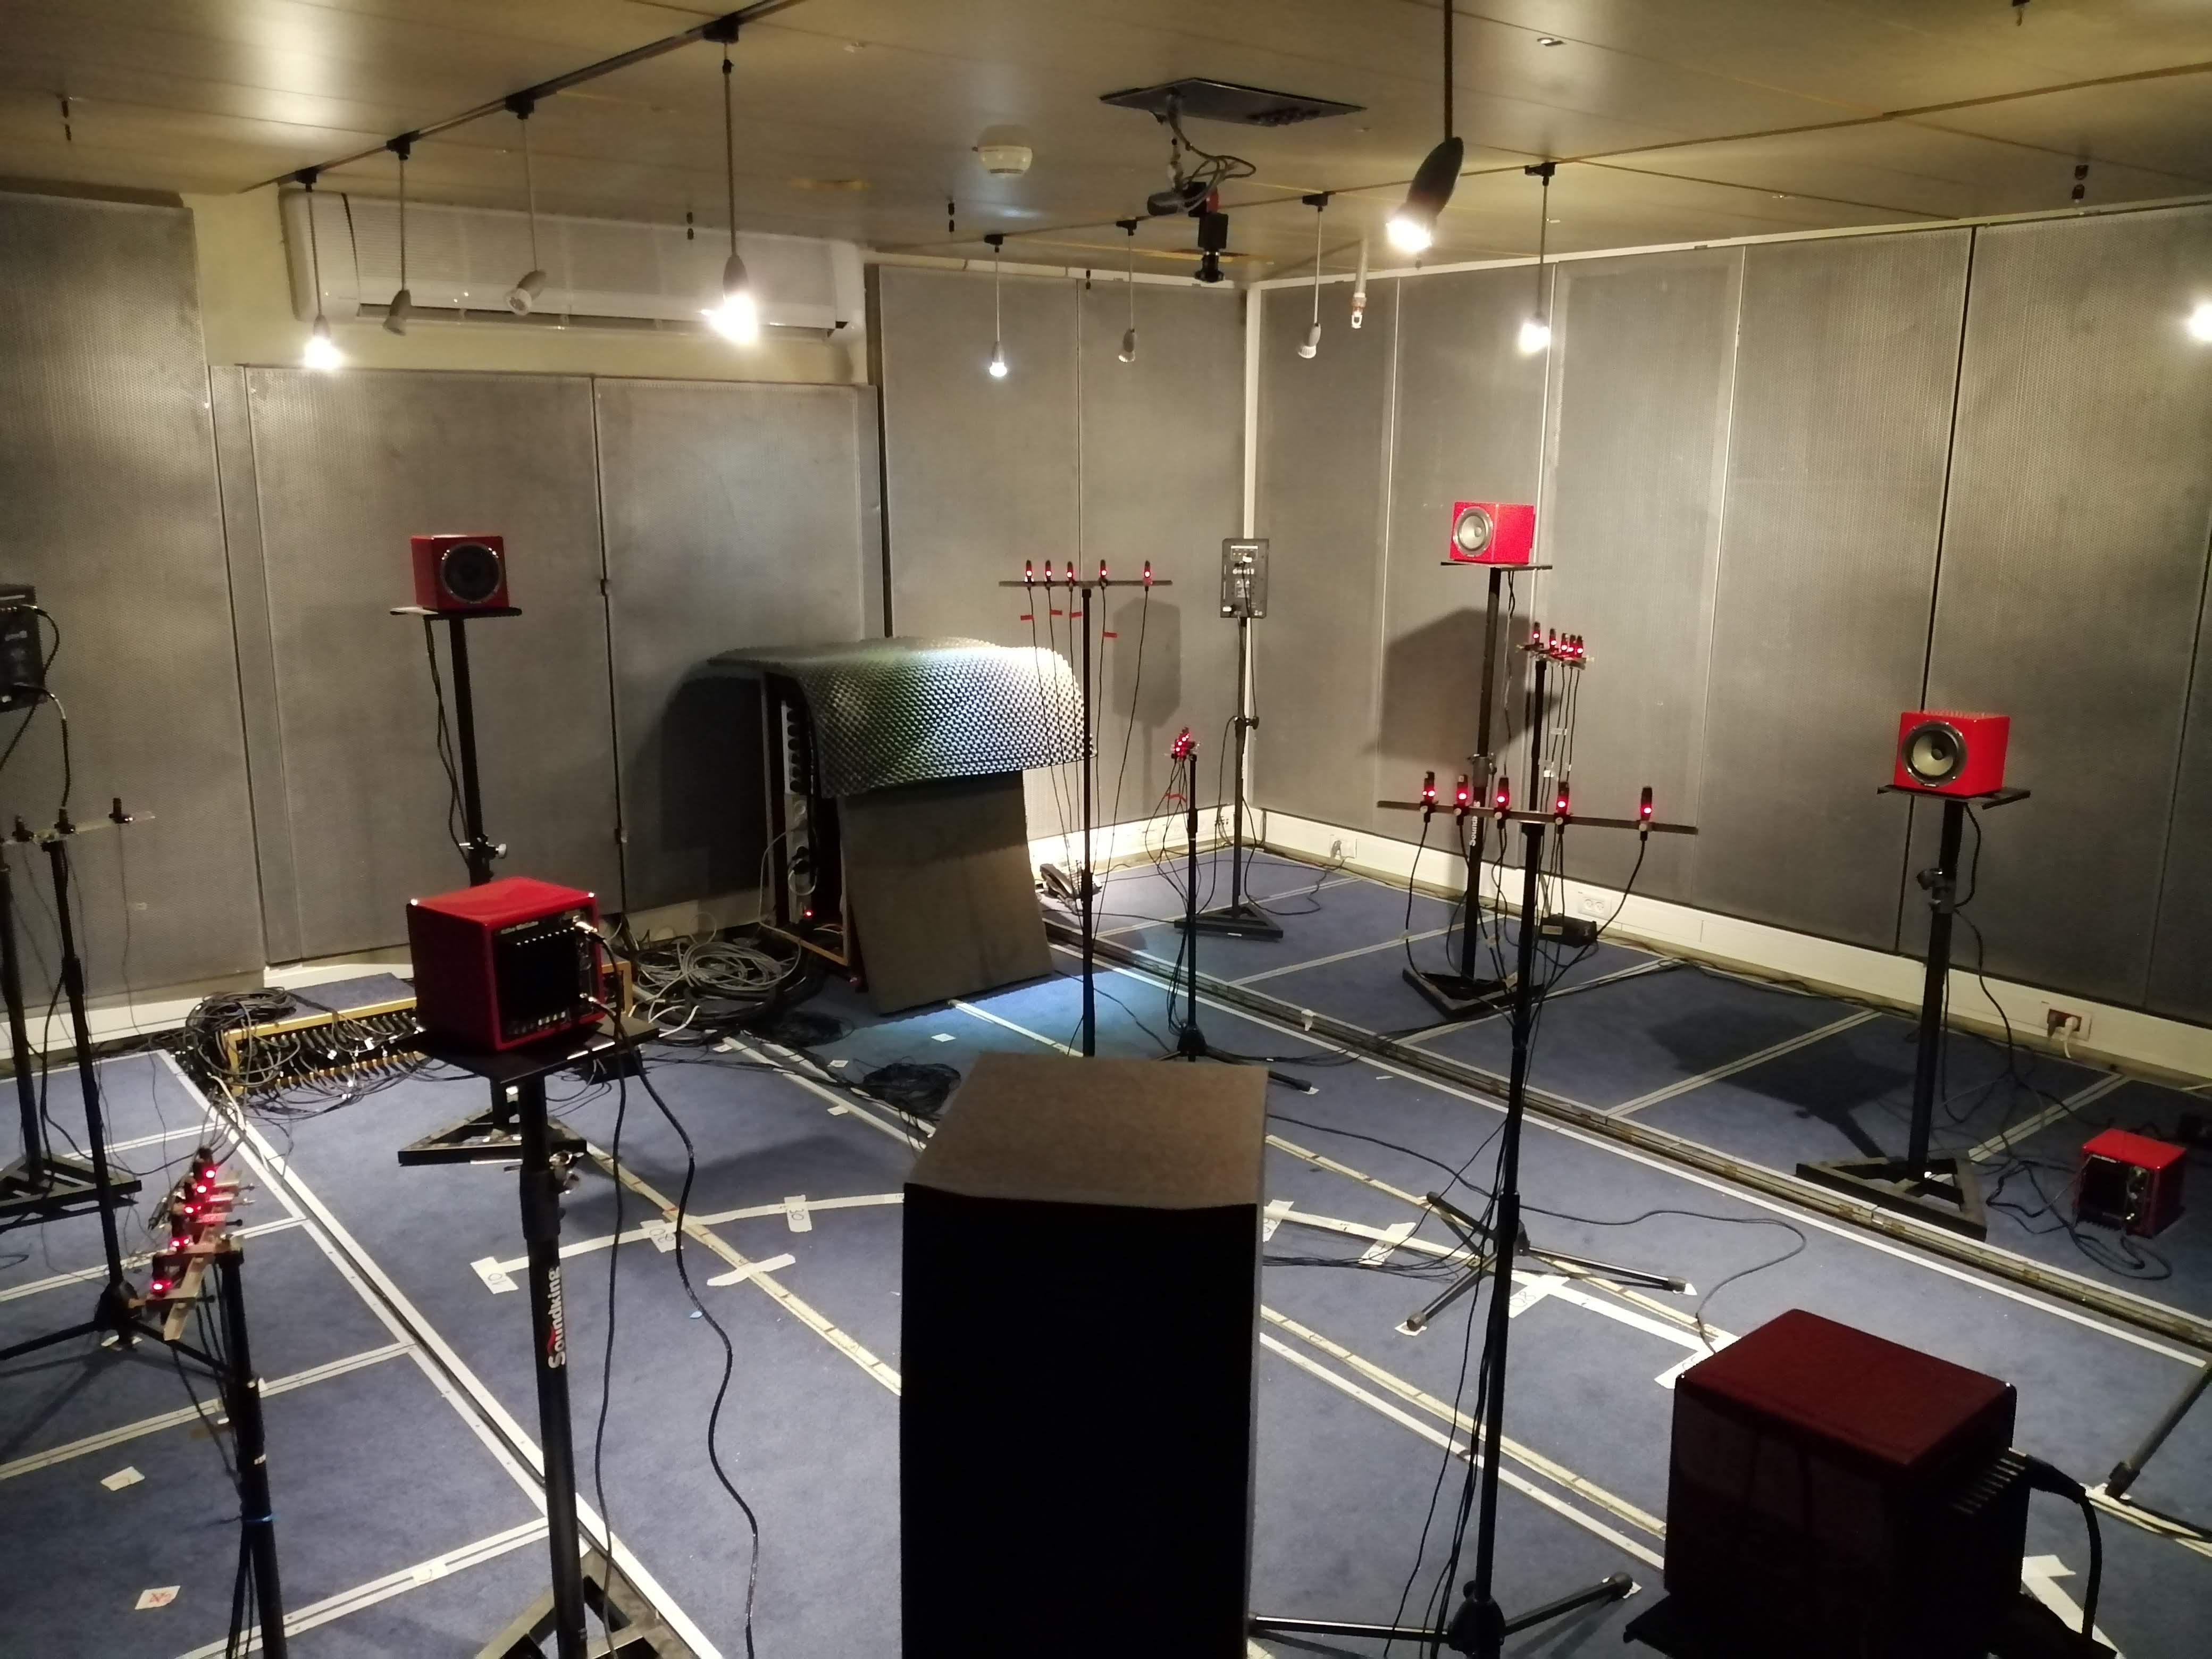
\includegraphics[width=0.325\textwidth]{figures/dechorate/recording_setup}}
    %
    \subfloat[mu_spkr][Microphone array]{
        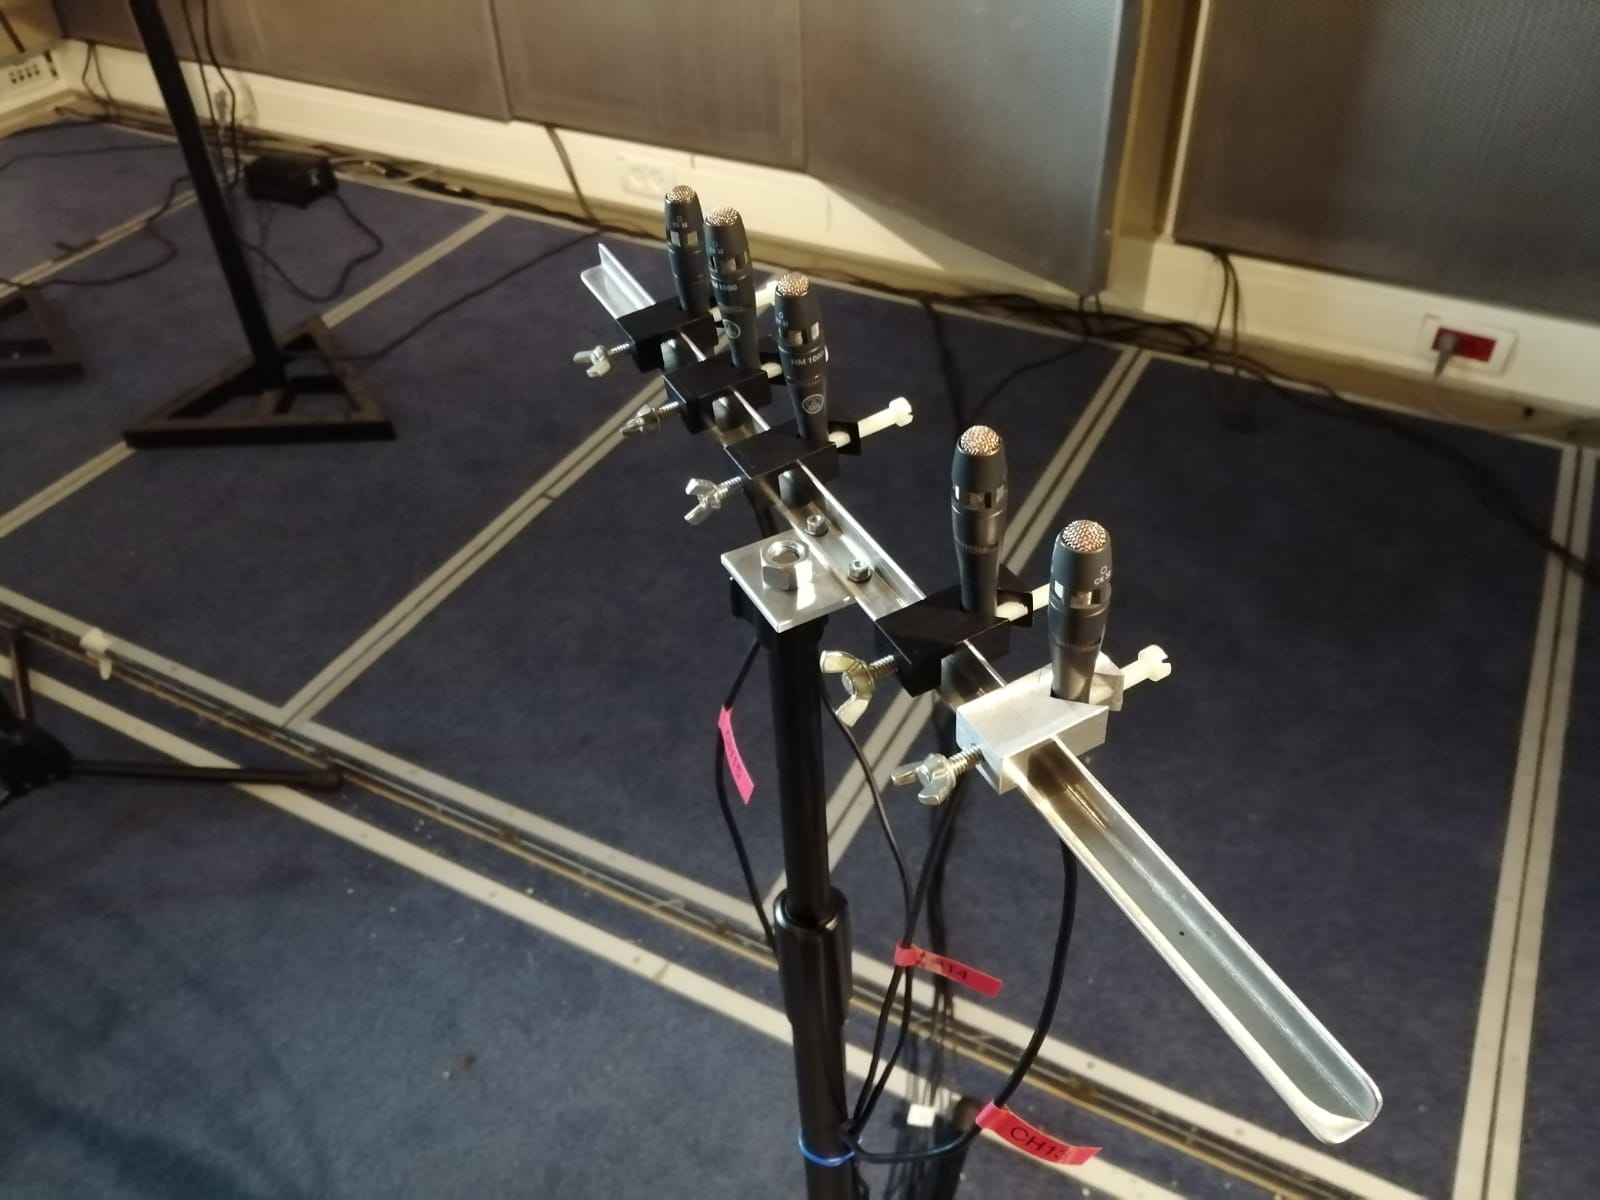
\includegraphics[width=0.325\textwidth]{figures/dechorate/mic}}
    %
    \subfloat[mu_univ][Revolving panels]{
            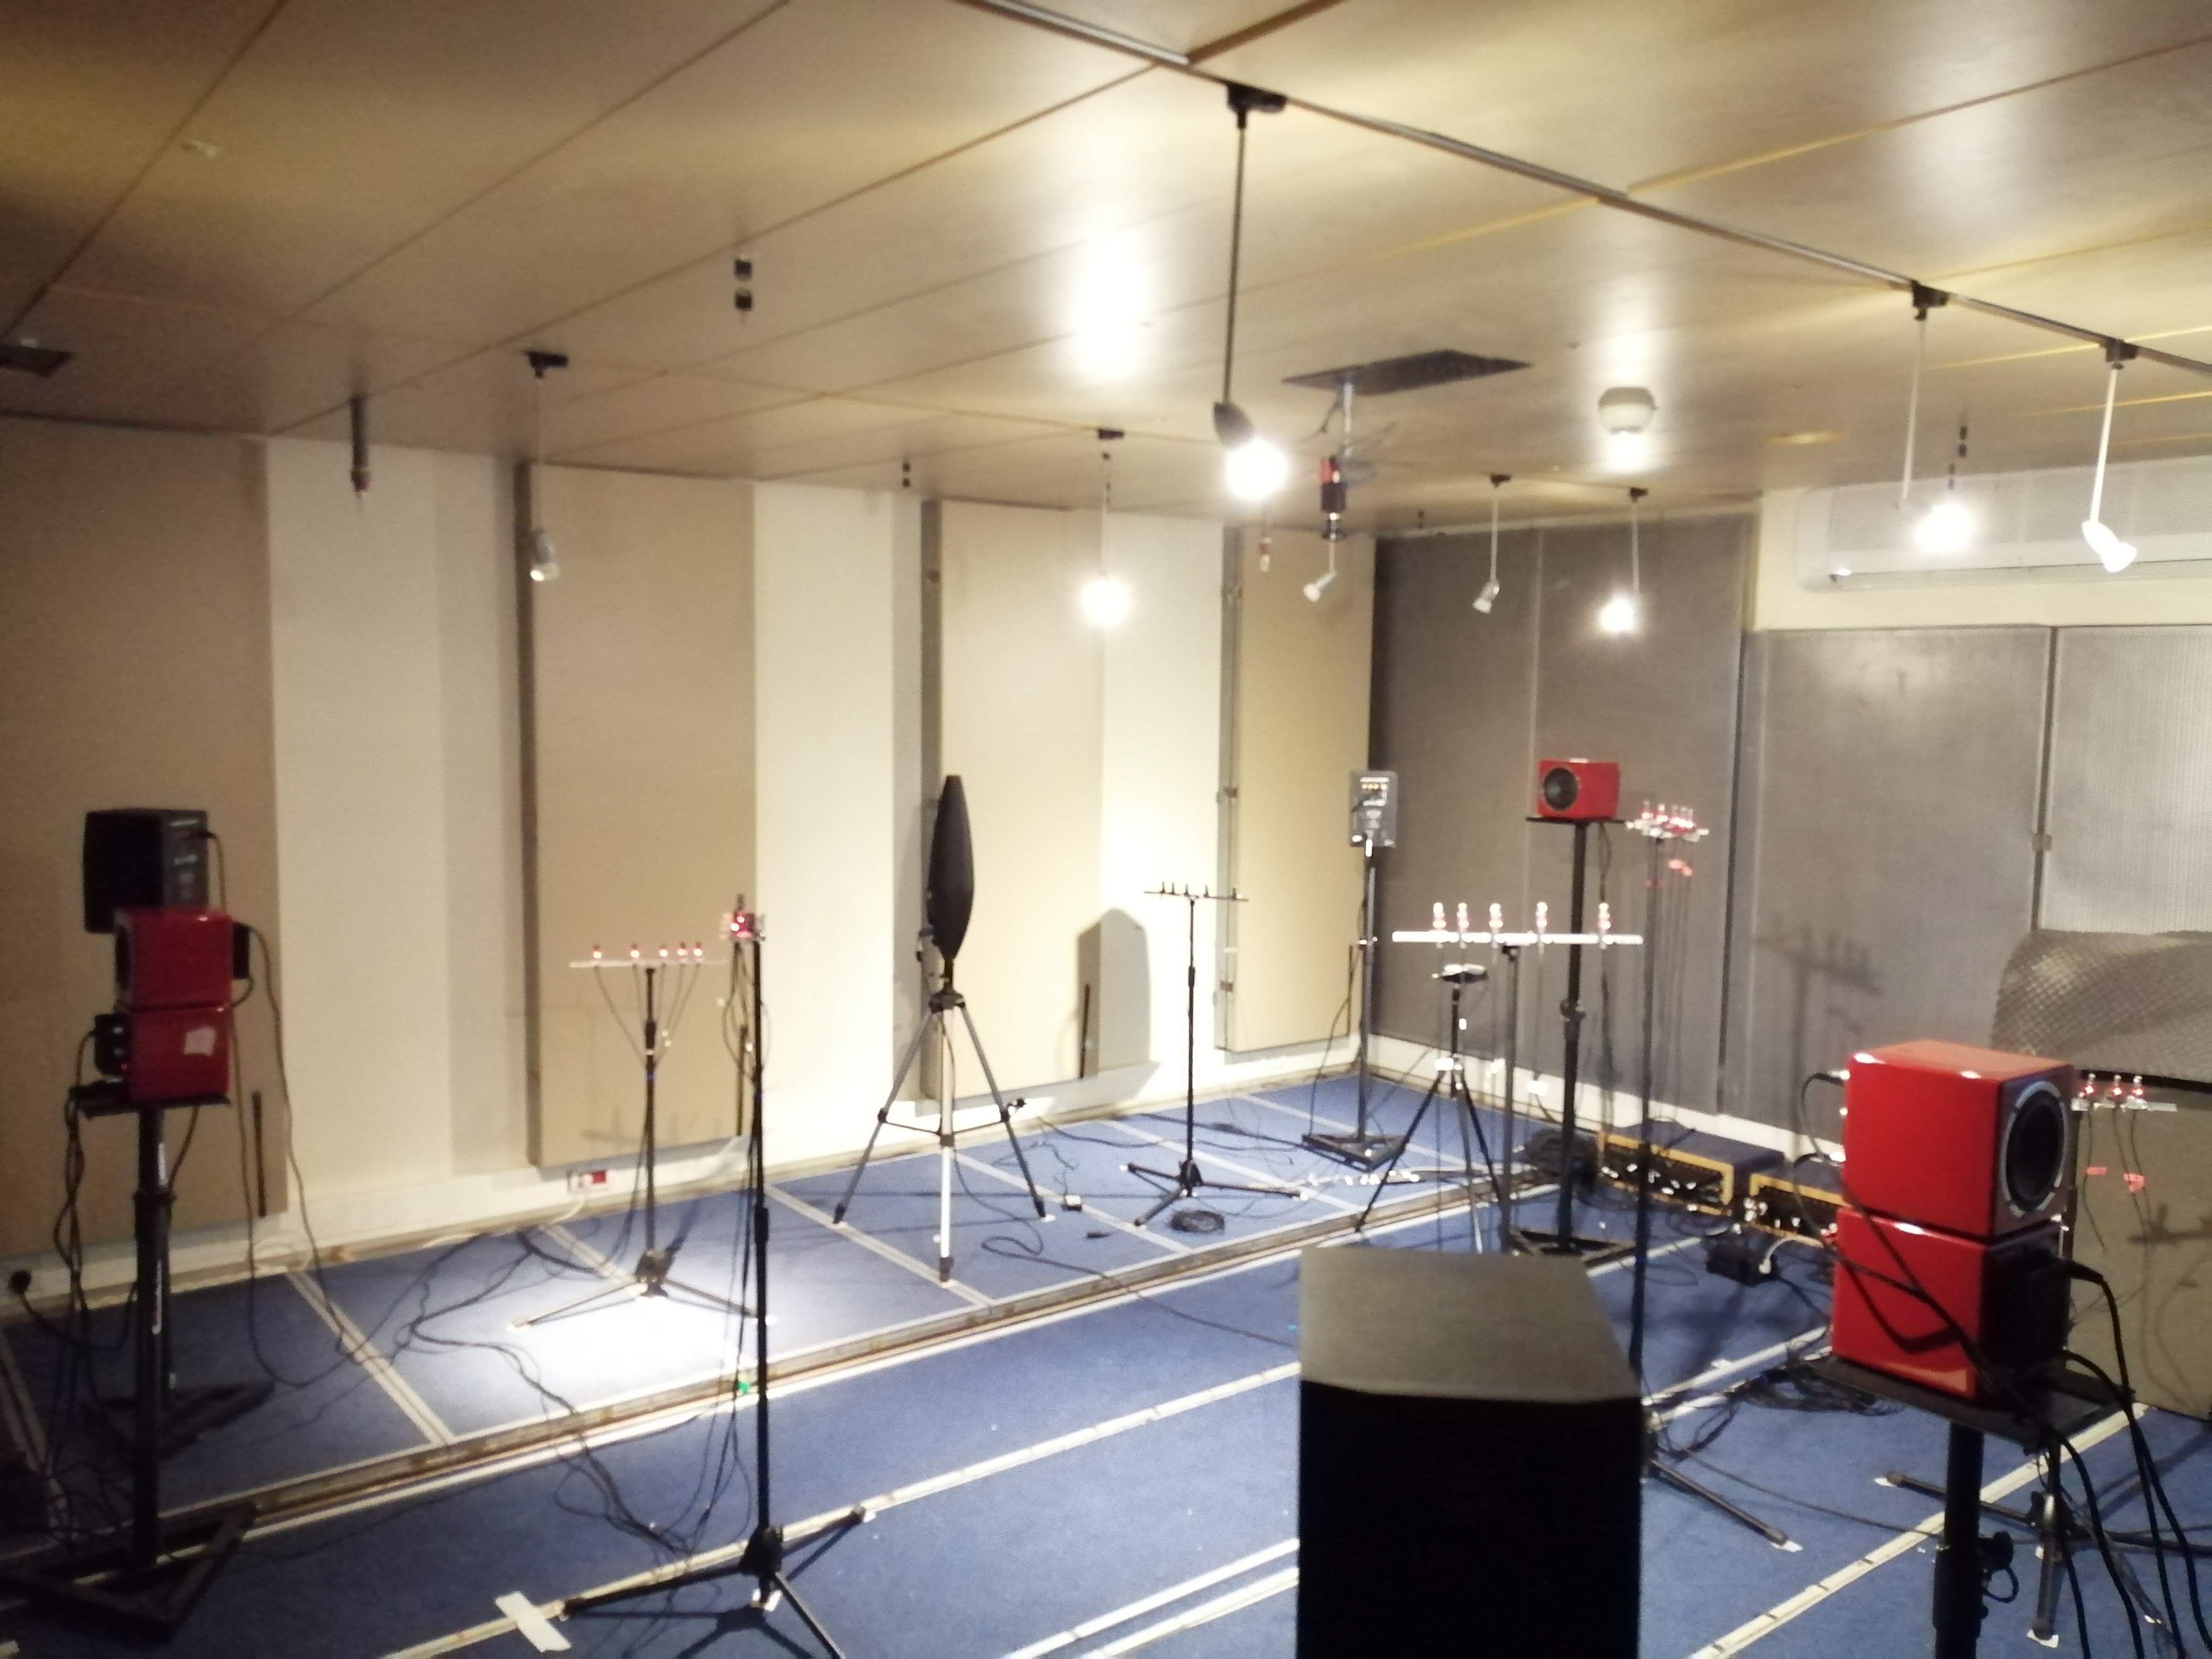
\includegraphics[width=0.325\textwidth]{figures/dechorate/panels}}
    \label{fig:dechorate:setup}
    \caption{Picture of the acoustic lab. From left to right: the overall setup, one microphone array, the setup with revolved panels.}
    \end{fullwidth}
\end{figure}

\subsection{Measurements}
The main feature of this room is the capability to change the acoustic profile of each of its facet by flipping double-sided panels with one reflective and one absorbing face.
This allows to achieve precise values of $\RT$ that range from 0.1 to almost 1~second.
In this dataset the panels of the floor were kept always absorbent.

\mynewline
Two types of sessions were considered, namely, \textit{one-hot} and \textit{incremental}.
For the first type, a single facet was placed in reflective mode while all the others were kept absorbent.
For the second type, starting from fully-absorbent mode, facets were progressively switched to reflective mode one after the other until all but the floor were reflective, as shown in Table \ref{tab:dechorate:wallcoding}.

\mynewline
The dataset features an extra recording session.
For this session, office furnitures were positioned in the room to simulate a typical meeting room with chairs and tables (See~\cref{fig:dechorate:room}).
Theses recordings will be used in future works for asserting the robustness of echo-aware methods in a more realistic scenario?.

\begin{table}[h]
    \begin{sidecaption}[]{
        Surface coding in the dataset: each binary digit indicates if the surface is absorbent ($\mathtt{0}$, \xmark ) or reflective ($\mathtt{1}$, \cmark).
        }[tab:dechorate:wallcoding]
        \centering
        \small
        \begin{tabular}{cc|cccccc}
\toprule
& Surfaces:                 & Floor                 & Ceiling               & West                  & South                 & East                  & North                 \\ \hline
\multicolumn{1}{c}{\multirow{5}{*}{\rotatebox{90}{one-hot}}} & $\mathtt{000000}$                   & \xmark & \xmark & \xmark & \xmark & \xmark & \xmark \\
& $\mathtt{010000}$                    & \xmark & \cmark & \xmark & \xmark & \xmark & \xmark \\
& $\mathtt{001000}$                    & \xmark & \xmark & \cmark & \xmark & \xmark & \xmark \\
& \multicolumn{1}{c|}{$\dots$}  & \multicolumn{6}{c}{$\dots$} \\
& $\mathtt{000001}$                    & \xmark & \xmark & \xmark & \xmark & \xmark & \cmark \\
\multicolumn{1}{c}{\multirow{4}{*}{\rotatebox{90}{incremental}}} & $\mathtt{011000}$                    & \xmark & \cmark & \cmark & \xmark & \xmark & \xmark \\
& $\mathtt{011100}$                    & \xmark & \cmark & \cmark & \cmark & \xmark & \xmark \\
& \multicolumn{1}{c|}{$\dots$} & \multicolumn{6}{c}{$\dots$}  \\
& $\mathtt{011111}$                    & \xmark & \cmark & \cmark & \cmark & \cmark & \cmark \\
\bottomrule
\end{tabular}


    \end{sidecaption}
\end{table}


\mynewline
For each room configuration and loudspeaker, three different excitation signals were played and recorded in sequence: chirps, white noise and speech utterances.
The former consists in a repetition of 3 \acf{ESS} signals of duration 10~seconds and frequency range from 100 Hz to 14~kHz interspersed with 2~seconds of silence.
Such frequency range was chosen to match the characteristics of the loudspeakers.
To prevent rapid phase changes and ``popping'' effects, the signals were linearly faded in and out over 0.2~seconds with a Tuckey taper window\sidenote{
    The code to generate the reference signals and to process them is available togheter with the data.
    Such code is based on the \href{https://github.com/maj4e/pyrirtool}{\library{pyrirtool}\ExternalLink} Python library.
}.
Secondly, 10~seconds bursts of white noise and 3 anechoic speech utterances from the \WSJ/ dataset \citeonly{Paul1992design} were reproduced in the room.
Through all the recordings, at least 40~dB of sound dynamic range was asserted and a room temperature of $\ang{24} \pm \ang{0.5}$ and humidity of 80\% were registered.
Moreover, 1~minute of \textit{room tone} (silence) and 4~minutes of diffuse babble noise were recorded for each session.
The latter was simulated by transmitting different chunks of the same single-channel babble noise recording from additional loudspeakers facing the four corners of the room.

\mynewline
All the microphone signals were synchronously acquired and digitally converted to 48 kHz with 32 bits/sample using the equipment listed in Table~\ref{tab:dechorate:room_equipment}. The polarity of each microphone was registered by clapping a book in the middle of the room.

\section{Dataset annotation}\label{sec:annotation}
\acp{RIR} are estimated with the ESS technique \citeonly{farina2007advancements} at 48 kHz:
the signal of a microphone recording an \ESS/ source is deconvolved by division in the frequency domain.
Notice that the \ac{FT} of the \ESS/ signal is available in closed form and we used its \ac{DFT} approximation.

\subsection{RIRs annotation}
The objective of this database is to feature off-grid annotations in the ``geometrical space'', namely microphone, wall and source positions, \textit{fully consistent} with annotations in the ``signal space'', namely the echo timings within the \acp{RIR}.
This results is achieved as follows:
\begin{enumerate}[label=(\roman*)]
    \item \label{it:decharate:ips} First, the ground-truth position of array and source centres are acquired via a Beacon indoor positioning system ($\bIPS$).
    This system consists in 4 stationary bases positioned at the corners of the ceiling and a movable probe used for measurements which can be located within errors of $\pm2$~cm.
    The elements of this system are shown in~\cref{fig:dechorate:bips}.
    \marginpar{
        \centering
        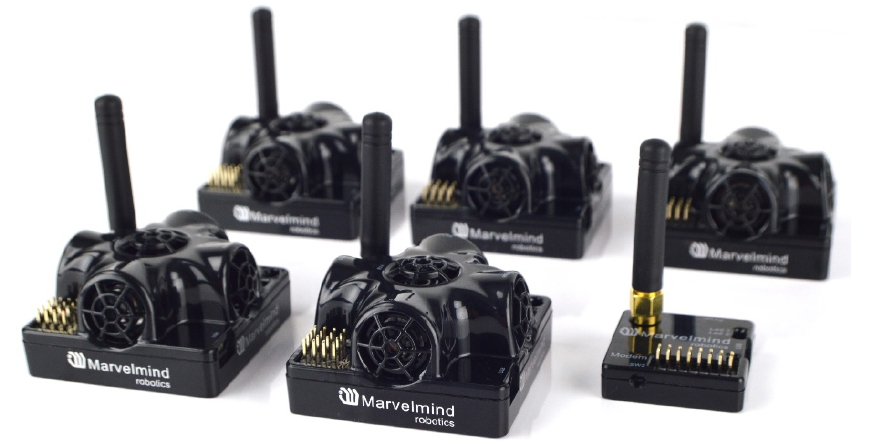
\includegraphics[width=\linewidth]{dechorate/IPSbeacon.jpg}
        \captionof{figure}{
            Picture of the Beacon indoor positioning system used for measuring array and loudspeaker 3D position.
        }
        \label{fig:dechorate:bips}
    }
    \item \label{it:decharate:not} The estimated \acp{RIR} are superimposed on synthetic \acp{RIR} computed with the \acf{ISM} from the geometry obtained in the previous step.
    A Python GUI\sidenote{This GUI is available in the dataset package.} (showed in~\cref{fig:dechorate:labelling_tools}), was used to manually tune a peak finder and label the echoes corresponding to found peaks, that is, annotate their positions and their corresponding image source position and wall label..

    \item \label{it:decharate:mds} By solving a simple \acf{MDS} problem \citeonly{dokmanic2015relax,crocco2016estimation, Plinge2016acoustic}, refined microphone and source positions were computed.
    The non-convexity of the problem was alleviated by using a good initialization (obtained at the previous step), by the high SNR of the measurements and, later, by including the additional image sources in the formulation.
    The prior information about the arrays' structures reduced the number of variables of the problem, leaving the 3D positions of the sources and of the arrays' barycenters in addition to the the arrays' tilt on the azimuthal plane.

    \item \label{it:decharate:lat} By employing a multilateration algorithm \citeonly{Beck2008ExactProblems}, where the positions of one microphone per array serve as anchors and the \TOAs/ are converted into distances, it was possible to localize image sources along side with the real sources.
    This step will be further discussed in~\cref{ch:dechorateapp}.
\end{enumerate}
Knowing the geometry of the recording room, we were able to manually label the echoes by iterating through steps \ref{it:decharate:not}, \ref{it:decharate:mds} and \ref{it:decharate:lat}.

\newthought{The final geometrical and signal annotation} was chosen as a compromise between the $\bIPS$ measurements and the \ac{MDS} output.
While the former ones are noisy but consistent with the scene's geometry, the latter ones matches the \TOAs/ but not necessarily the physical world.
In particular, geometrical ambiguities such as global rotation, translation and up-down flips were observed.
Instead of manually correcting this error, we modified the original problem from using only the direct path distances ($\dMDS$) to considering the  image sources' \TOA/ of the ceiling as well in the cost function ($\dcMDS$).
Table~\ref{tab:dechorate:res_mds} shows numerically the \textit{mismatch} (in cm) between the geometric space (defined by the $\bIPS$ measurements) and the signal space (the one defined by the echo timings, converted in cm).
To better quantify it, we introduce here a \textit{goodness of match} (GoM) metric: it measures the fraction of (first-order) echo timings annotated in the \acp{RIR} matching the annotation produced by the geometry within a threshold.
Including the ceiling information, $\dcMDS$ produces a geometrical configuration which has a small mismatch (0.41~cm in average) in both the signal \textit{and} geometric spaces with $98.1\%$ of matching first order echoes within a 1~ms threshold.
Nevertheless, it is interesting to see that the $\bIPS$ measurements produce a good but less precise annotation.

\begin{table}[]
    \begin{sidecaption}[]{
        Mismatch between geometric measurements and signal measurements in terms of maximum (Max.), average (Avg.) and standard deviation (Std) of absolute mismatch in centimeters. The \textit{goodness of match} (GoM) between the signal and geometrical measurements is reported as fraction of matching echo timing for different threshold in milliseconds.
        }[tab:dechorate:res_mds]
        \centering
        \small
        \begin{tabular}{lllll}
\toprule
& Metrics        & $\bIPS$               & $\dMDS$          & $\dcMDS$          \\
\midrule
\multicolumn{1}{c}{\multirow{2}{*}{\rotatebox{90}{\footnotesize Geom.}}}
&   Max.             & -            & $6.1$         & $1.07$        \\
&   Avg.$\pm$Std.    & -            & $1.8\pm1.4$    & $0.39\pm0.2$  \\
% \rule{0pt}{0.1em}\\
\midrule
\multicolumn{1}{c}{\multirow{2}{*}{\rotatebox{90}{\footnotesize Signal}}}
&   Max.          & $5.86$         & $1.20$         & $1.86$       \\
&   Avg.$\pm$Std. & $1.85\pm 1.5$  & $0.16\pm0.2$   & $0.41\pm0.3$ \\
% \rule{0pt}{0.1em}\\
\midrule
\multicolumn{1}{c}{\multirow{3}{*}{\rotatebox{90}{\footnotesize Mismatch}}}
&  GoM (1.0 ms)   & $97.9 \%$      & $93.4 \%$      & $98.1 \%$ \\
&  GoM (0.1 ms)   & $26.6 \%$      & $44.8 \%$      & $53.1 \%$ \\
&  GoM (0.05 ms)  & $12.5 \%$      & $14.4 \%$      & $30.2 \%$ \\
\bottomrule
\end{tabular}

    \end{sidecaption}
\end{table}

\subsection{Other tools for RIRs annotation}
Finally, we want to mention that the following tools and techniques were found helpful in annotating the echoes.

\newthought{The \library{skyline} visualization} consists in presenting multiple \acp{RIR} as an image, such that the wavefronts corresponding to echoes can be highlighted \citeonly{Baba2018b}.
More precisely, it is the visualization of the $L \times N$ matrix $\mathbf{H}$ created by stacking column-wise $N$ normalized echograms\sidenote{
    The echogram is defined either as the absolute value or as the squared value of the \ac{RIR}.
}, that is $\mathbf{H}_{l, n} =\bar{\eta}_{n}(l) = \kvbar{h_{n}(l)}/\max{\kvbar{h_{n}(l)}}$, where $l = 0, \dots, L-1$ is  the sample index and $n$ is an arbitrary indexing of all the microphones for a fixed room configuration.
4 \ac{RIR} \library{skyline}s for 4 directional sources for the full reflective scenario are shown in Figure~\ref{fig:dechorate:skyline}, stacked horizontally, preserving the order of microphones within the arrays.
The reader can notice several clusters of 5 adjacent bins of similar color (intensity) corresponding to the arrivals at the array's sensors.
Thanks to the usage of linear arrays, this visualization allowed us to identify both \TOAs/ and their labeling.

\begin{figure}[h]
    \begin{sidecaption}[]{
        Detail of the GUI used to manually annotate the \acp{RIR}.
        For a given source and microphone,
        a) and b) shows 2 \RIRs/ for 2 different room walls configuration (blue and orange) before and after the direct path deconvolution respectively.
        c) shows the results of the peak finder for one of the deconvolved RIRs, and d) is a zoom on the \ac{RIR} \library{skyline} (See \cref{fig:dechorate:skyline}).
        }[fig:dechorate:labelling_tools]
    \centering
    \small
    \begin{overpic}[width=\linewidth]{figures/dechorate/labeling_tool.pdf}
        \put (2,   195) {\footnotesize a)}
        \put (160, 195) {\footnotesize b)}
        \put (2,   95)  {\footnotesize c)}
        \put (160, 95)  {\footnotesize d)}
    \end{overpic}
    \end{sidecaption}
    \label{}
\end{figure}


\begin{figure}
    \begin{sidecaption}[]{
        \ac{RIR} \texttt{Skyline} annotated with observed peaks ($\times$) together with their geometrically-expected position ($\circ{}$) computed with the \library{Pyroomacoustic} simulator.
        As specified in the legend, different colors are used to indicate the room facets responsible for the reflection: direct path ($\mathtt{d}$), ceiling ($\mathtt{c}$), floor ($\mathtt{f}$), west wall ($\mathtt{w}$), $\dots$, north wall ($\mathtt{n}$).
    }[fig:dechorate:skyline]
    \centering
    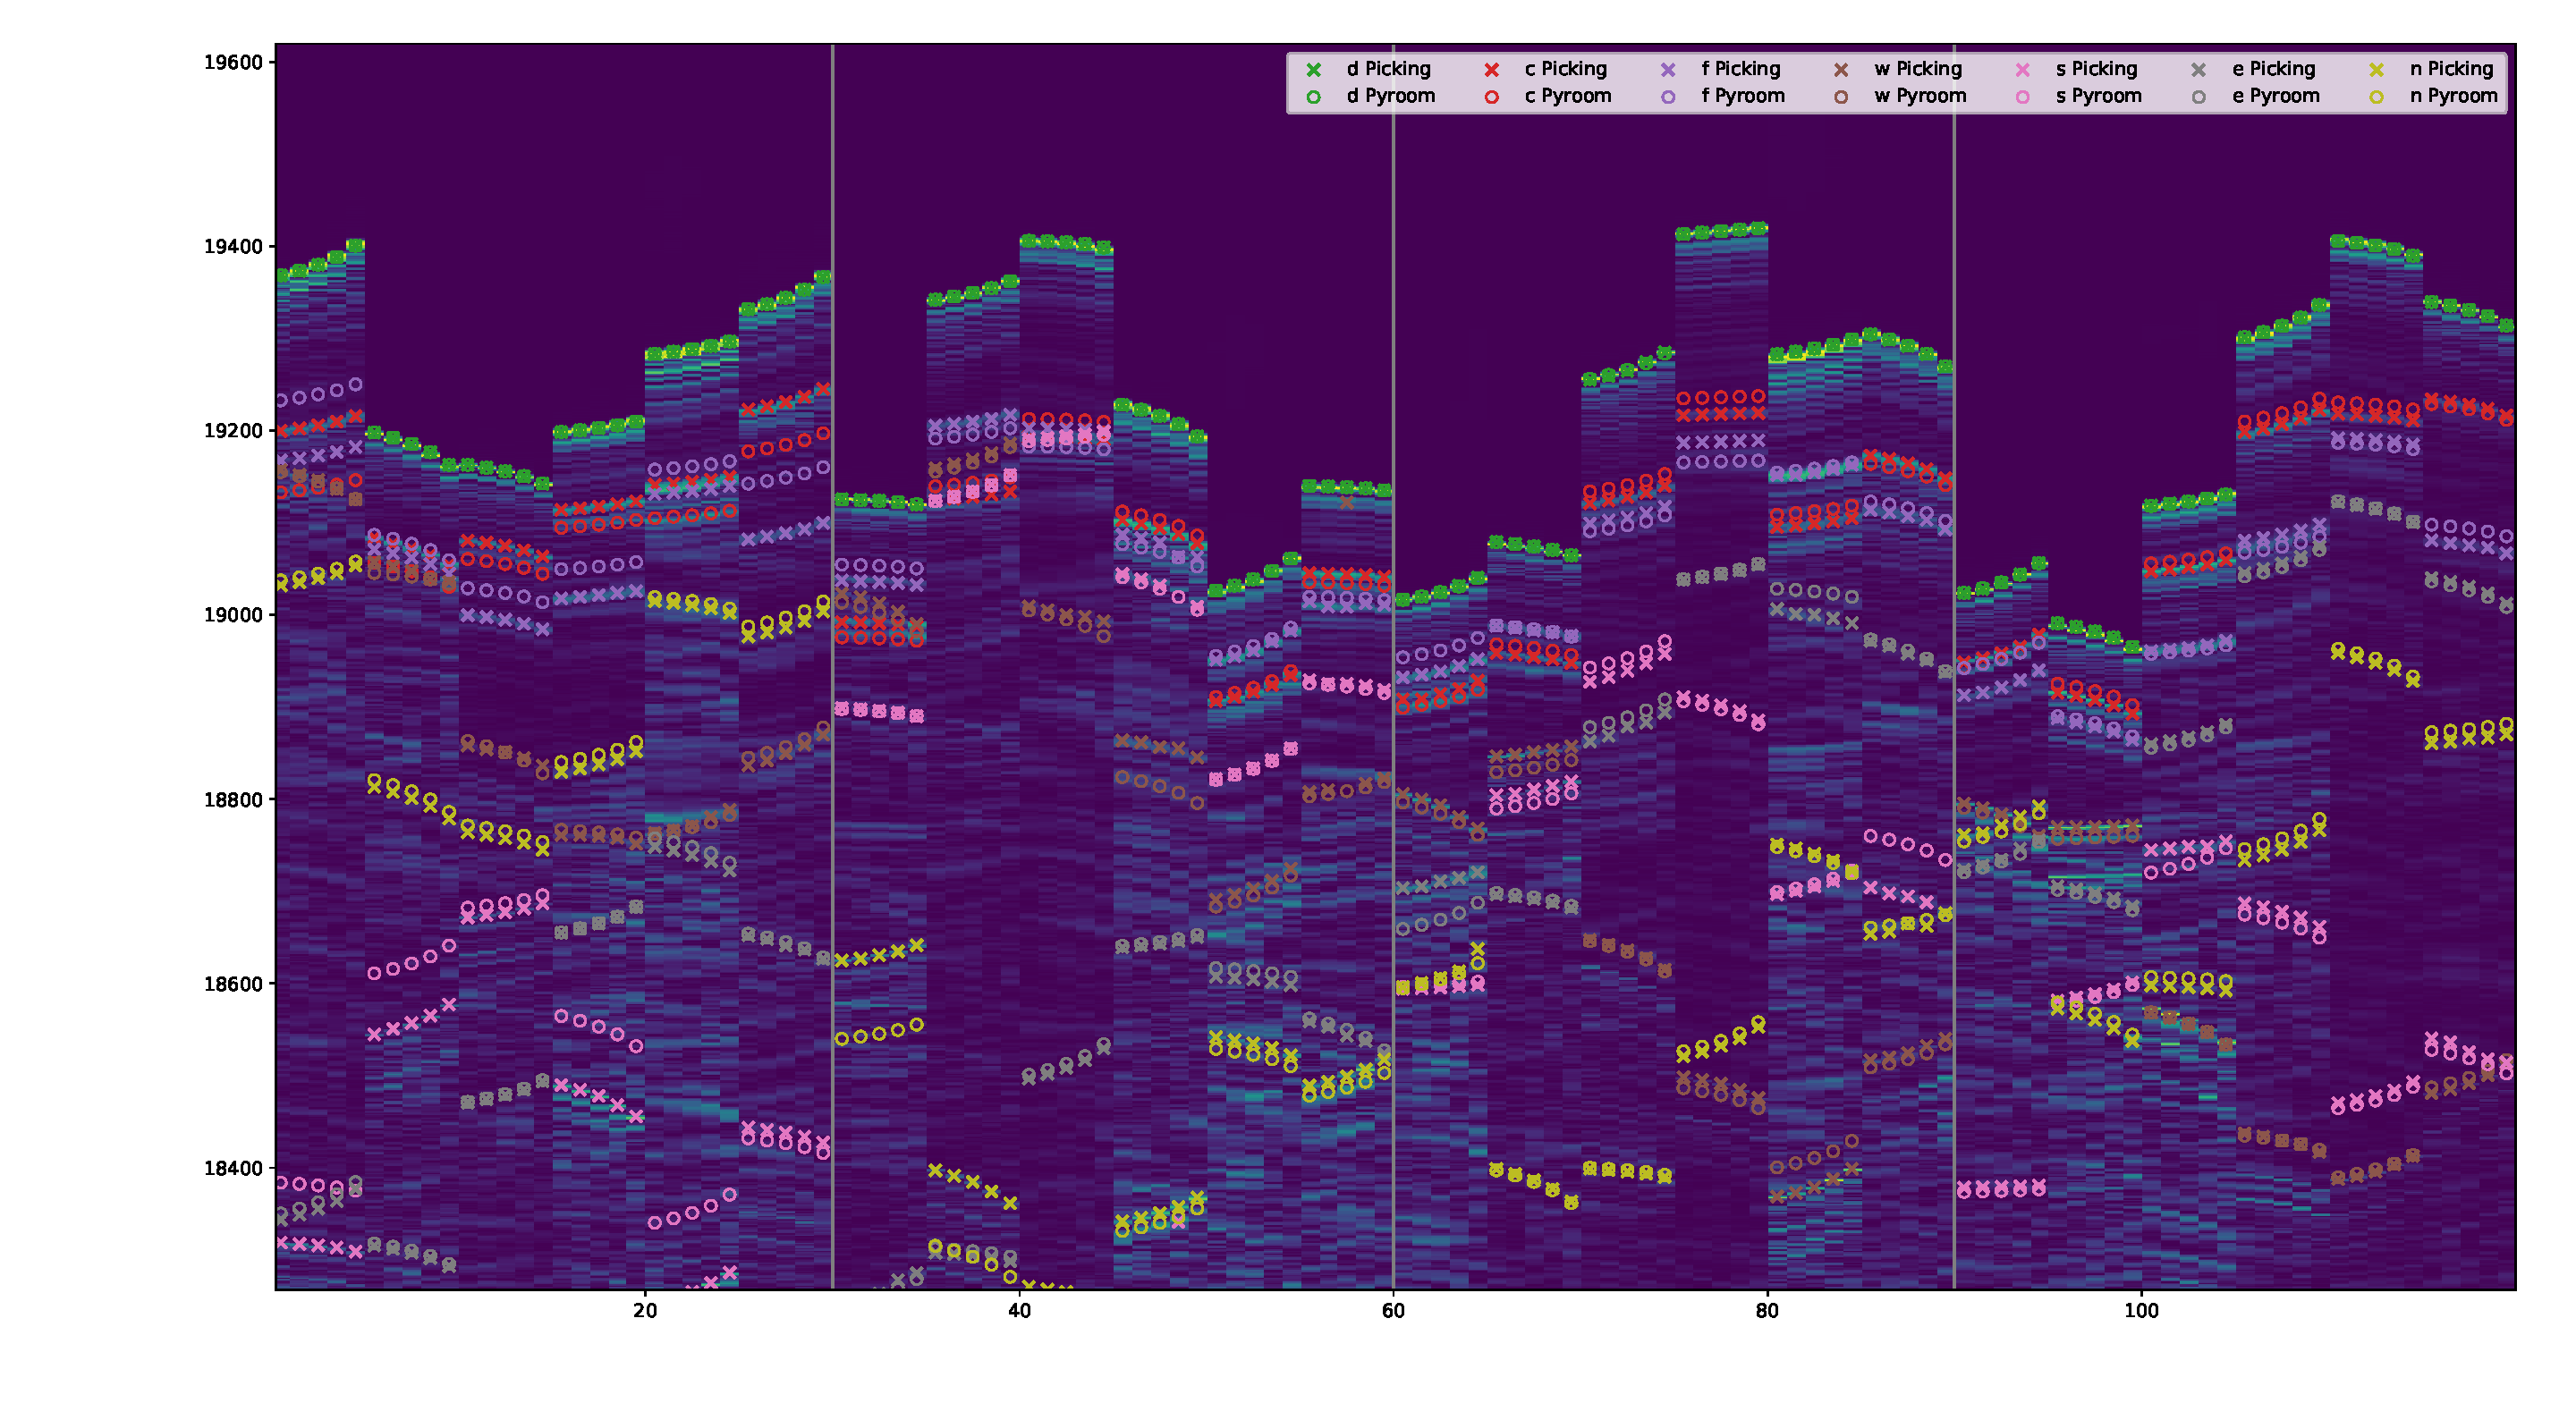
\includegraphics[trim={15em 15em 2em 0},clip,width=\linewidth]{figures/dechorate/rir_skyline_final_mod4paper.pdf}
    \end{sidecaption}
\end{figure}

\newthought{Direct path deconvolution/equalization} was used to compensate the frequency response of the source loudspeaker and microphone \citeonly{antonacci2012inference, Eaton2016estimation}.
In particular, the direct path of the RIR was manually isolated and used as an equalization filter to enhance early reflections from their superimposition and from background noise before proceed with peak picking.
Each \ac{RIR} was equalized with its relative direct path.
As depicted in Figure~\ref{fig:dechorate:labelling_tools}, in some situation this process was necessary for correctly identifying the underlying \TOAs/' peaks.

\newthought{Different wall configurations} for the same geometry influenced the peaks' predominance in the \ac{RIR}, hence facilitating its echo annotation.
An example of \acp{RIR} corresponding to 2 different surface configurations is shown in~\cref{fig:dechorate:labelling_tools}: the reader can notice how the peak predominance changes for the different configurations.

\newthought{An interpolation-based peak finder}\sidenote{
    In this work, peaks are found using the Python \href{https://bitbucket.org/lucashnegri/peakutils/}{\library{peakutils}\ExternalLink} library.
} was used on equalized echograms $\bar{\eta}_{n}(l)$ to provide an initial guess on the peak positions.

\subsection{Limitations of current annotation}
As stated in \citeonly{defrance2008finding}, we want to emphasize that annotating the correct \TOAs/ of echoes and even the direct path in ``clean'' real \acp{RIR} is far from straightforward.
The peaks can be blurred out by the loudspeaker characteristics or the concurrency of multiple reflections.
However as showed in~\cref{fig:dechorate:skyline}, the proposed annotation was found to be sufficiently consistent both in the geometric and in the echo space.
Thus, no further refinement was done.
This database can be used as a first basis to develop better \AER/ methods which could be used to iteratively improve the annotation, for instance including  2$^\text{nd}$ order reflections.

\section{The \library{dEchorate} package}
The dataset comes with both data and code to parse and process it.
The data are presented in 2 modalities: the \texttt{raw} data, that is, the collection of recorded wave files, are organized in folders and can be retrieved by querying a simple database table; the \texttt{processed} data, which comprise the estimated \acp{RIR} and the geometrical and signal annotations, are organized in tensors directly importable in Matlab or Python (\textit{e.g.} all the \acp{RIR} are stored in a tensor of dimension $L \times I \times J \times D$, respectively corresponding to the RIR length in samples, the number of microphones, of sources and of room configurations).
\\Together with the data a Python package is available on the same website.
This includes wrappers, GUI, examples as well as the code to reproduce this study.
In particular, all the scripts used for estimating the \acp{RIR} and annotating them are available and can be used to further improve and enrich the annotation or as baselines for future works.

\begin{figure}
    \begin{sidecaption}[]{
            Sample view of the database table to retrieve the raw wave file and its attributes.
        }[fig:dechorate:dataset]
        \centering
        
\includegraphics[width=\linewidth]{figures/dechorate/database.png}
    \end{sidecaption}
\end{figure}

\conclusion{This work} introduced a new database of \RIRdef/ featuring accurate annotation of early echoes and microphone positions.
These data can be used to test methods in the room geometry estimation pipeline and in echo-aware audio signal processing.
We will show some application in \SE/ and \RooGE/ in~\cref{ch:dechorateapp}.
\qed